 \documentclass[addpoints]{exam}
\usepackage{url}
\usepackage{amsmath,amsthm,enumitem}
\usepackage{amssymb}
\usepackage{graphicx}
\usepackage{xcolor}
\usepackage{algpseudocode}
\usepackage{algorithm}
\usepackage{units}
%\input myfonts

\newtheorem*{claim}{Claim}
\title{CS 6150 - Fall 2025 - HW2\\Greedy algorithms, Local search, Graph traversal \& shortest paths}
\date{Submission date:  Friday, Oct 31, 2025 (11:59 PM)}

% \def\mysolution#1{#1} % Uncomment this to reveal answers
\def\mysolution#1{}    % Uncomment this to hide answers 

\begin{document}
\maketitle
\begin{center}
\fbox{\fbox{\parbox{5.5in}{\centering
This assignment has \numquestions\ questions, for a total of \numpoints\
points. You will still be graded out of 100, and any points you earn above 100 will count as bonus and can compensate for a low score on other homeworks.
Unless otherwise specified, complete and reasoned arguments will be expected for all answers. }}}
\end{center}

\qformat{Question \thequestion: \thequestiontitle\dotfill \textbf{[\totalpoints]}}
\pointname{}
\bonuspointname{}
\pointformat{[\bfseries\thepoints]}


\begin{center}
  \gradetable
\end{center}
\newpage

{\setlength{\parindent}{0cm} \textbf{Note: Unless otherwise specified, complete and well-reasoned arguments for correctness and running time are expected for all answers. For the problems based on graphs, the different graph algorithms we covered in class (breadth-first/depth-first traversal, Dijkstra, Bellman-Ford, etc.) can be used as black-boxes if you apply them directly as we learned them. However, if you modify them to suit a given problem, spell out the modifications clearly (i.e. they are no longer black-boxes) with their effect on correctness and running time. Assume that, by default, $n$ represents the number of vertices while $m$ represents the number of edges in a graph.}}\\\\

\begin{questions}
\titledquestion{Santa's tradeoffs}[15]
Recall the matching problem we saw in class: there are $n$ gifts, and $n$ children,
and each child has a non-negative valuation for each gift. Formally, the value of
gift $j$ to child $i$ is given by $V_{i,j}$. We assume that all $V_{i,j} \ge 0$.
Santa's goal is to give one gift to each child, so as to maximize the {\em total
value} (of course, a gift cannot be given to more than one child).
Suppose we now perform a more elaborate local search, this time picking every {\em
triple} of edges in the current solution, and seeing if there is a reassignment of
gifts between the end points of these edges that can improve the total value. Prove
that a locally optimal solution produced this way has a value that is at least two-thirds ($\nicefrac{2}{3}$) of the optimum value. [This kind of trade-off is typical in local search --
each iteration is now more expensive ($O(n^3)$ instead of $O(n^2)$), but the
approximation ratio is better.]\\

\textbf{To start this proof assume we begin with a locally optimum solution. This means that no swaps of three pairs will result in a higher happiness score. To demonstrate the relationship that comes from this assume we have 5 kids $i,j,k,l,m$ the correspodning gifts for those 3 kids are $a,b,c,d,e$. Our goal here is to compare the locally optimum solution to the global. When comparing our solutions let $j$ be the child that receives $a$'s global optimal gift, $k$ be the child that receives $j$'s global optimal gift, $d$ be the child that recieves $c$'s global optimal gift, and finaly let $e$ be the child that receives $m$'s global optimal gift. the illustration below demonstrates this relationship}
 \begin{figure}[H]
 \centering
  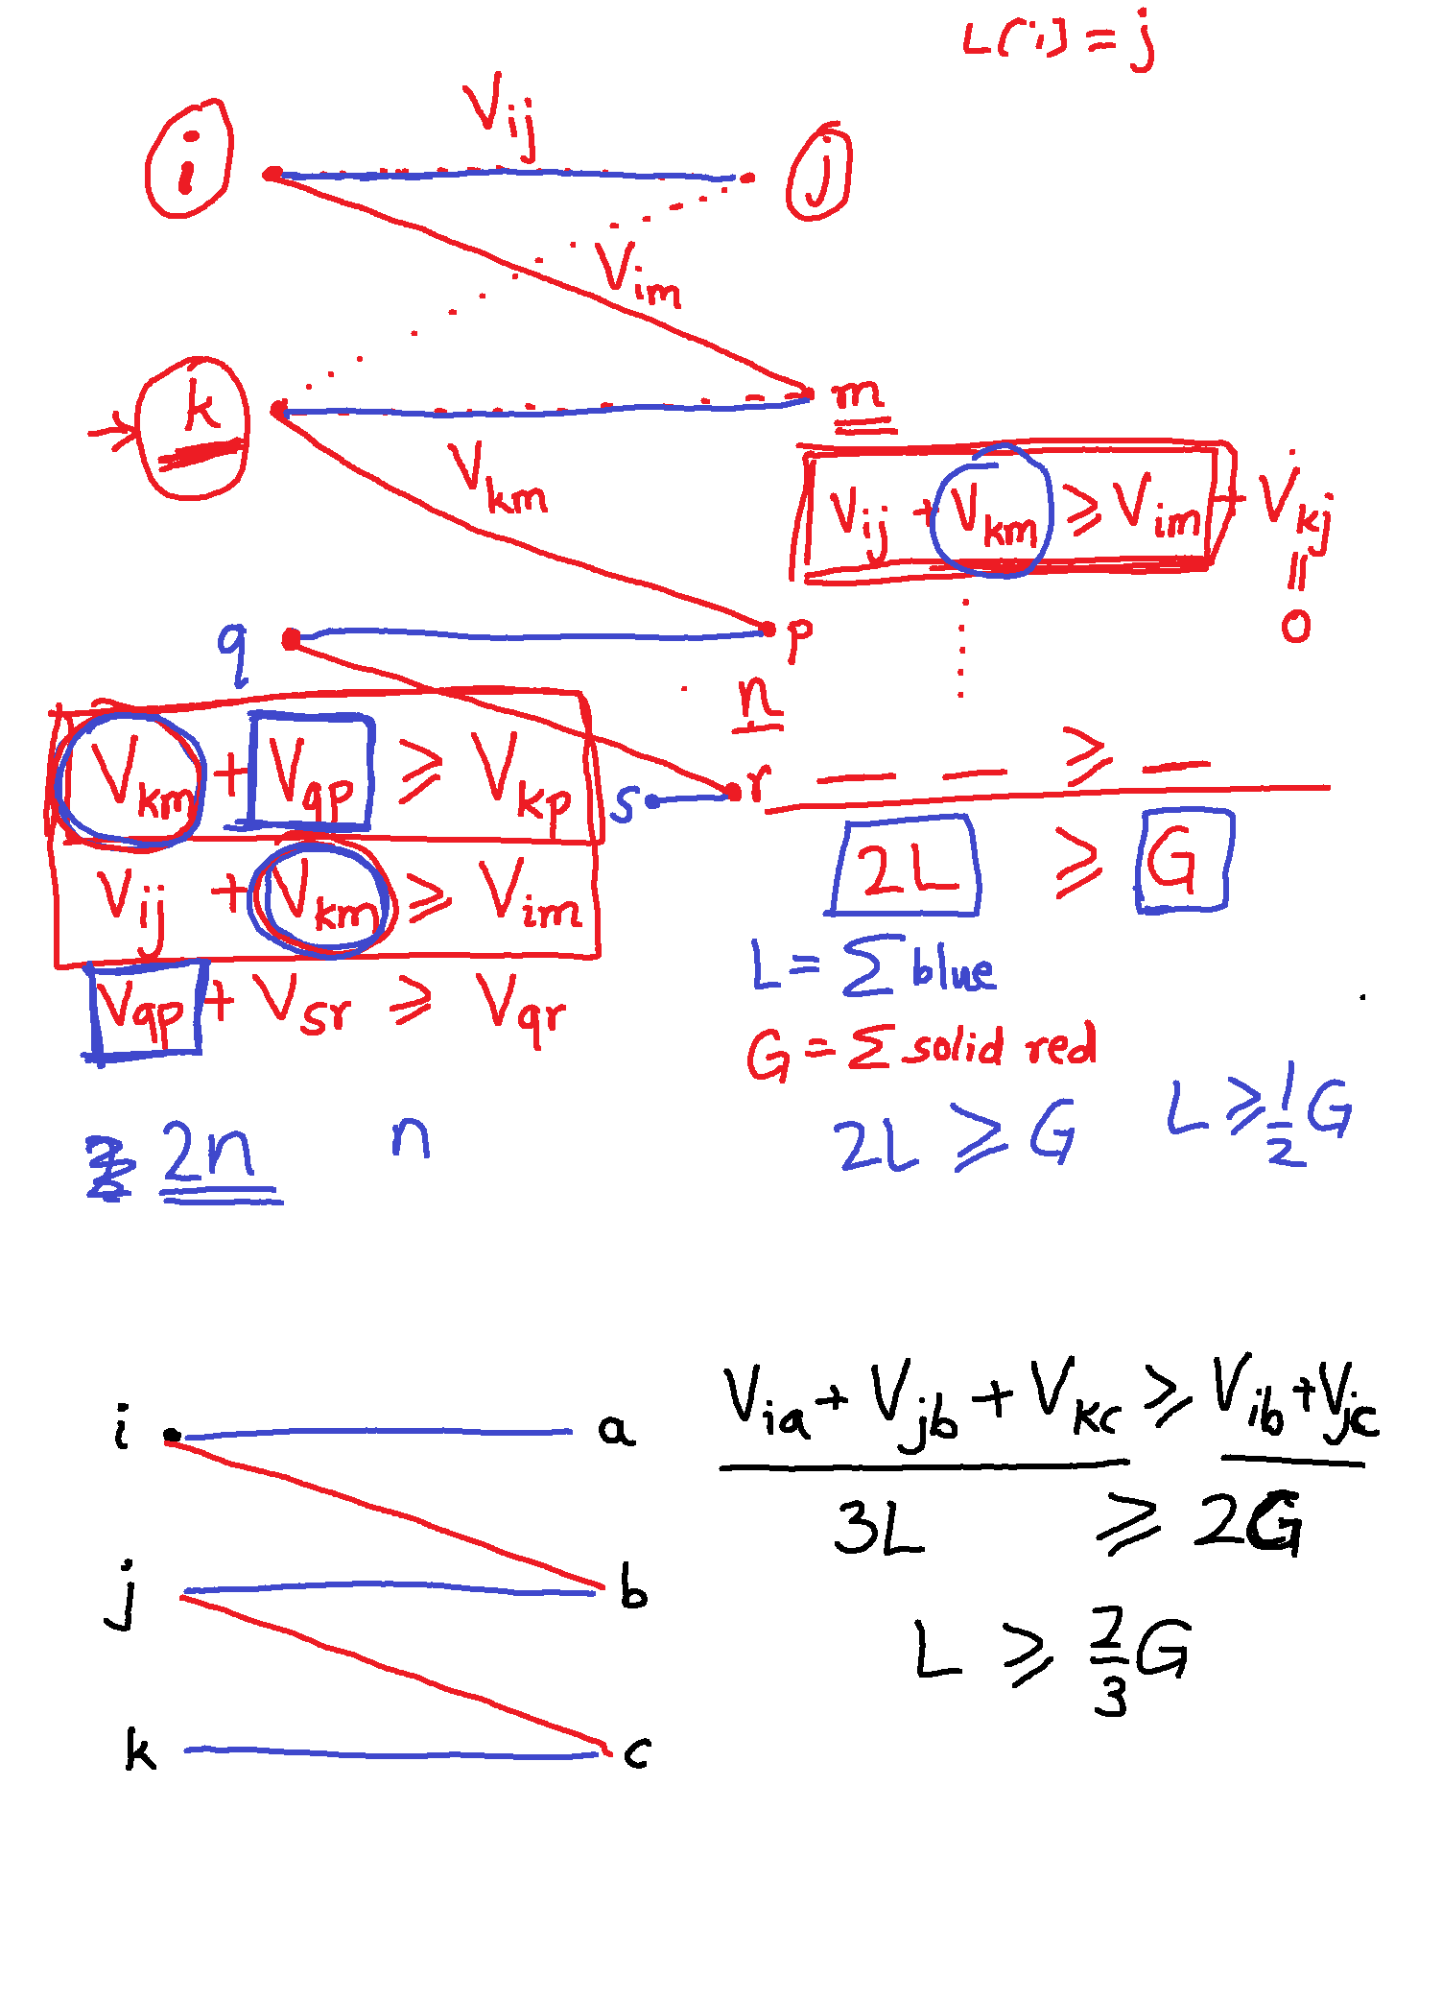
\includegraphics[width=0.3\textwidth]{Gift Giving.png}
 \caption{Diagram of Relationship As Requested By Yash}
 \end{figure}

\textbf{Using this information we can get innequalities that will allow us to compare our two solutions.}

\textbf{$V_{i,a} + V_{j,b} + V_{k,c} \ge V_{i,b} + V_{j,c} + V_{k,a}$ With our current problem structure we don't have any information on the happiness of $V_{k,a}$ so we will simply consider the worst case where the happiness received from the mapping of $V_{j,a}$ is $0$. Another thing to remember here is that $i$'s optimal gift is $b$ and $j$'s optimal gift is c}

\textbf{Using the same logic we can do the next level of the innequalities which would result in $V_{j,b} + V_{k,c} + V_{l,d} \ge V_{j,c} + V_{k,d} + V_{l,b} \rightarrow V_{j,b} + V_{k,c} + V_{l,d} \ge V_{j,c} + V_{k,d}$}

\textbf{To make the pattern clear we will go one more level. $V_{k,c} + V_{l,d} + V_{m,e} \ge V_{k,d} + V_{l,e}$. Once again we consider the worst case for the last gift.}

\textbf{Putting all of these innequalities together show us the pattern that will allow us to finish our proof}

\textbf{Let $\sigma_i$ represent the locally optimum gift for child $i$}

\textbf{Let $\gamma_i$ represent the globally optimum gift for child $i$}
\begin{align}
    V_{i,a} + V_{j,b} + V_{k,c} &\ge V_{i,b} + V_{j,c} \\
    V_{j,b} + V_{k,c} + V_{l,d} &\ge V_{j,c} + V_{k,d} \\ 
    V_{k,c} + V_{l,d} + V_{m,e} &\ge V_{k,d} + V_{l,e} \\ 
    & ... \\
    \hline \\  
    \sum_{i=1}^{n}(V_{i,\sigma_i}) + \sum_{j=1}^{n}(V_{j,\sigma_j}) + \sum_{k=1}^{n}(V_{k,\sigma_k}) &\ge \sum_{i=1}^{n}(V_{i,\gamma_i}) + \sum_{j=1}^{n}(V_{j,\gamma_j}) 
\end{align}

\textbf{From this we can see that each edge in the locally optimum solution appears $3$ times the left hand side and each edge in the globally optimum solution appears $2$ times on the right hand side. This pattern will continue for all children gift pairs so long as they are setup as above. We also notice that each summation on the left hand side is equivalent and each summation on the right hand side is equivalent. A simplified expression for what this means is shown below}

\begin{align}
    3L \ge 2G
\end{align}
\textbf{Where $L$ is the locally optimal solution and $G$ is the globally optimal solution. If we simplify this expression we get that}

\begin{align}
    L \ge \frac{2}{3}G
\end{align}

\textbf{Therefore we have proven that a locally optimal solution produced this way has a value that is at least two-thirds the optimum value.}
\mysolution{
    \input{Sol-1}
}



\titledquestion{$t$ farthest elements from each other}
A common problem in returning search results is to display results that are {\em diverse}. A simplified formulation of the problem is as follows. We have $n$ points in Euclidean space of $d$-dimensions, and suppose that by distance, we mean the standard Euclidean distance. The goal is to pick a subset of $t$ (out of the $n$) points, so as to maximize the sum of the pairwise distances between the chosen points. 
I.e., if the points are denoted $P = \{p_1, p_2, \dots, p_n\}$, then we wish to choose an $S \subseteq P$, such that $|S| = t$, and $\sum_{p_i, p_j \in S} d(p_i, p_j)$ is maximized.

A common heuristic for this problem is local search. Start with some subset of the points, call them $S = \{q_1, q_2, \dots, q_t\} \subseteq P$. At each step, we check if replacing \underline{one of the $q_i$} with a point in $P \setminus S$ improves the objective value.  If so, we perform the swap, and continue doing so as long as the objective improves. The procedure stops when no improvement (of this form) is possible. Suppose the algorithm ends with $S = \{q_1, \dots, q_t\}$.  We wish to compare the objective value of this solution with the optimum one. Let $\{x_1, x_2, \dots, x_t\}$ be the optimum subset. 

\begin{parts}
\part[5]  Use local optimality to argue that:
\[ d(x_1, q_2) + d(x_1, q_3) + \dots + d(x_1, q_t) \le d(q_1, q_2) + d(q_1, q_3) + \dots + d(q_1, q_t). \]

\textbf{This innequality comes from reasoning about the global optimum and the local optimum. As in the problem statement lets define the global optimum to be $x_1, x_2, ..., x_t$ and the local optimum to be $q_1, q_2, ..., q_t$}

\textbf{first define $d(x,y)$ to be the distance between $x$ and $y$. We know by the definition of local optimality that:}
\[\sum(d(x_i, x_j) \ge \sum(d(q_i,q_j)))\]

\textbf{Or in words that the global optimum must be $\ge$ local optimum. Now lets look at the case where we swap one of the options in our local optimum $q_1$ for something in our global opimum $x_1$. We can use the second part of the definition of local optimality to argue the innequality below. Noting that by locality any swap of the pairs in the local optimum will not result in a better result}
\[
\sum(d(\text{swapped}) \le \sum(d(q_i,q_j)))
\]
\textbf{We can expand this innequality as follows. Starting with the left hand side}
\[
d(x_1,q_2) + d(x_1,q_3) + ... + d(x_1,q_t) + d(q_2, q_3) + d(q_2, q_4) + ... + d(q_2, q_t) + ... ... + d(q_{t-1}, q_t)
\]
\textbf{Next we can expand the left hand side}
\[
d(q_1,q_2) + d(q_1,q_3) + ... + d(q_1,q_t) + d(q_2, q_3) + d(q_2, q_4) + ... + d(q_2, q_t) + ... ... + d(q_{t-1}, q_t)
\]
\textbf{If we look at both sides together we realize that there are many repeated terms on each side of the innequality. Using algebra we can cancel these duplicates out and are left with the following innequality.}
\[ d(x_1, q_2) + d(x_1, q_3) + \dots + d(x_1, q_t) \le d(q_1, q_2) + d(q_1, q_3) + \dots + d(q_1, q_t). \]
\textbf{This is exactly the innequality we were trying to argue so the proof is complete.}
\mysolution{
\input{Sol-2a}
}

\part[8] Deduce that:  [{\em Hint:} Use two inequalities of the form above.]
\[ (t-1) \cdot d(x_1, x_2) \le 2 \left[ d(q_1, q_2) + d(q_1, q_3) + \dots + d(q_1, q_t) \right]. \]
\textbf{The first thing to notice here is the term $d(x1,x2)$. With our current equations we don't really have any information on the distances between the optimal. Because of this we need to use a fact that is true for all Euclidean distances. We will use the triangle innequality.}
\[d(x_1,x_2) \le d(x_1, q_j) + d(q_j, x_2)\]
\textbf{When we are doing our distances comparisons we compare the point with every other point than itself so we can generalize this to all points}
\begin{align}
(t-1)d(x_1,x_2) \le \sum_{j=2}^td(x_1, q_j) + \sum_{j=2}^td(q_j, x_2) \tag{*} 
\end{align}
\textbf{We can now introduce the information we learned from (a) to reason about those two sums}
\[\sum_{j=2}^td(x_1, q_j) \le \sum_{j=2}^td(q_1, q_j)\]
\[\sum_{j=2}^td(x_2, q_j) \le \sum_{j=2}^td(q_1, q_j)\]
\textbf{Simply plugging in those new innequalities into (*) we get the innequality asked for. These are strictly greater than the quantities in (*) so plugging them in doesn't ruin the innequality}
\begin{align*}
(t-1) \cdot d(x_1, x_2) \le 2 \left[ d(q_1, q_2) + d(q_1, q_3) + \dots + d(q_1, q_t) \right]. \tag{f\_b}
\end{align*}
\setcounter{equation}{0}
\mysolution{
\input{Sol-2b}
}

\part[10] Use this expression to argue that 
\[ \sum_{i,j} d(x_i, x_j) \le 2 \sum_{i,j} d(q_i, q_j).\]
Note: this shows that the local optimum has an objective value at least $\nicefrac{1}{2o}$ the global optimum.

\textbf{We will start by generalizing the left hand side of the equation $f_b$. To do this we will count how many terms will appear if we apply the left hand side to all points in the global optimum. If we expand out the summation we notice this pattern}
\begin{align*}
d(x_1, x_2), d(x_1, x_3), d(x_1, x_4), ... \\ 
             d(x_2, x_3), d(x_2, x_4), ... \\
                          d(x_3, x_4), ... \\ 
                                     , ...
\end{align*}
\textbf{Counting the number of terms that appear and noticing arithmetic series}
\begin{align*}
t - 1 \\ 
t - 2 \\ 
... \\
= \frac{(t-1) * t}{2} \tag{**}
\end{align*}

\textbf{We can now fully generalize the left hand side taking special care to remember how many terms came from that expansion so we can later apply it to the right hand side}
\[
(t-1) \sum_{i,j} d(x_i, x_j)
\]

\textbf{Because of the form of $f\_b$ for every term of the sum of the left hand side we get the right hand side.}
\begin{align*}
    (t-1) * \sum_{i,j}d(x_i, x_j) \le \frac{(t-1) * t}{2} * 2 * \sum_{j=2}^{t} d(q_1,q_j)
\end{align*}
\textbf{Note: The first term in the equation comes from the count analysis in (**). The summation comes from the right hand side of $f\_b$ taking special care to remember that the equation only considers distances from $q_1$. Simplifying the equaiton gives:}
\begin{align*}
    \sum_{i,j}d(x_i, x_j) \le t \sum_{j=2}^{t} d(q_1,q_j)
\end{align*}
\textbf{We now want to generalize the right hand side to all pairs $(q_k,q_j)$ do this by summing over all t}

\begin{align*}
    \sum_k^t \sum_{i,j}d(x_i, x_j) \le \sum_k^t t \sum_{j=2}^{t} d(q_k,q_j) \\
    t * \sum_{i,j} d(x_i, x_j) \le t \sum_k^t \sum_{j=2}^{t} d(q_k,q_j) \\
    \sum_{i,j} d(x_i, x_j) \le \sum_k^t \sum_{j=1}^{t} d(q_k,q_j) \\
    \sum_{i,j} d(x_i, x_j) \le \sum_{k,j}^{t} d(q_k,q_j) \\
\end{align*}
\textbf{Note that the summation in the last equation starts at $j=1$ rather than $j=2$ this is because when we generalize we need to consider $q_1$ with every other gift}
\textbf{When we do the summation on right side we get the following}
 \begin{figure}[H]
 \centering
  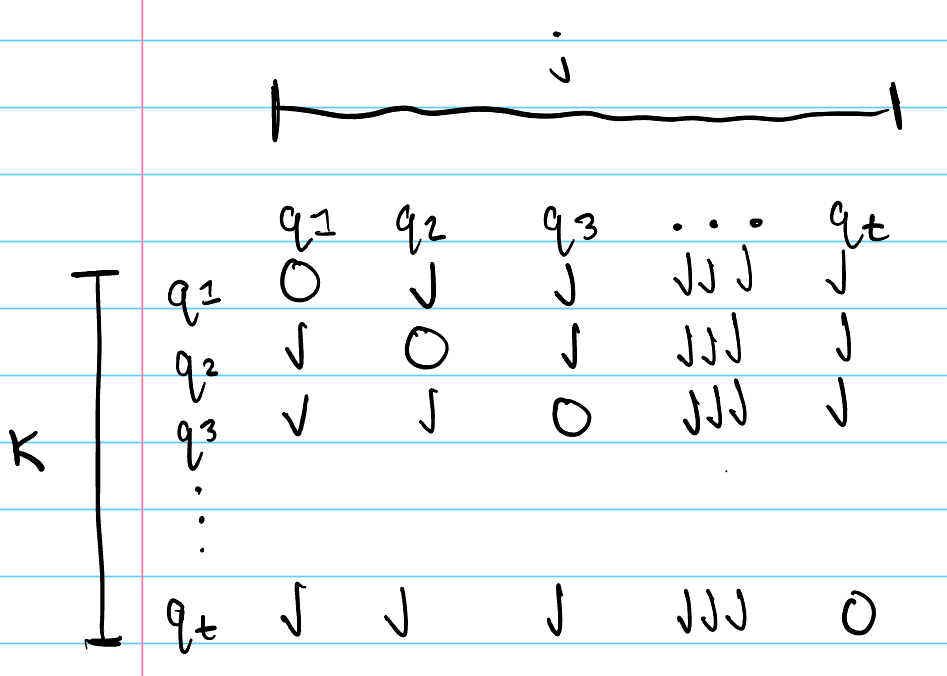
\includegraphics[width=0.5\textwidth]{RHS expansion.png}
 \caption{Table Expansion of Right Hand Side}
 \end{figure}

\textbf{The checkmarks represent the entries that are included for each row and the cirlces represent the ones that are excluded (they are excluded because they were already taken care of)}

\textbf{We notice that every pair $(q_k,q_j)$ appears twice once in the form $(q_k,q_j)$ and in the form $(q_j, q_k)$. This gives the following}
\begin{align*}
\sum_{i,j} d(x_i, x_j) \le 2 * \sum_{k,j}^{t} d(q_k,q_j) \\
\end{align*}

\textbf{Therefore we have found the innequality that was asked for and we know that the local optimum has an objective value at least $\frac{1}c{2}$ the global optimum}
\mysolution{
\input{Sol-2c}
}
\end{parts}
\newpage
\titledquestion{Set Cover Revisited}
In class, we saw the set cover problem (phrased as picking the smallest set of people who cover a given set of skills). Formally, we have $n$ people, and each person has a subset of $m$ skills. Let the set of skills of the $i$th person be denoted by $S_i$, which is a subset of $[m]$ (shorthand for $\{1, 2, \dots, m\}$). 
\begin{parts}
\part[8] Suppose that there is a set of seven (7) people whose skill sets optimally cover all of $[m]$ (i.e., together, they possess all the skills). Now, suppose we run the greedy algorithm discussed in class until the set of people chosen covers at least $75\%$ of the skills. How many people must we pick using the greedy algorithm to ensure this coverage?

\textbf{In class we proved the following theorem}

\textbf{Suppose there is an optimum solution that uses $k$ people. Then the greddy algorihtm does not use more than $k\log_{e}{m}$ people. This argument came from the fact that at every step the number of uncovered skills followed this innequality}
\[u_{t+1} \le u_t - \frac{u_t}{k}\]
\textbf{Follwoing this innequality through all steps we get the following}
\[u_{t+1} \le u_0(1-\frac{1}{k})^{t+1}\]
\textbf{We know the value of $k=7$}
\[u_{t+1} \le u_0(\frac{6}{7})^{t+1}\]
\textbf{We know that we want to cover $75\%$ of the skills so that means when we are done we only want $25\%$ of the skills to be uncovered.}
\[u_{t} \le m(\frac{6}{7})^{t} \le 0.25m\]
\[u_{t} \le (\frac{6}{7})^{t} \le 0.25\]
\textbf{Simply solve for t}
\[(\frac{6}{7})^{t} \le 0.25\]
\[t \le \frac{\log(0.25)}{\log(\frac{6}{7})} \approx 8.99 \]
\textbf{Because we add a new person at each iteration we know that you must add $9$ people to to cover at least $75\%$ of the skills}

\mysolution{
\input{Sol-3a}
}

\part[6] Consider the following ``street surveillance'' problem. We have a graph $(V, E)$ with $n$ nodes and $m$ edges. We are allowed to place surveillance cameras at the nodes. Once placed, they can monitor all the edges incident to the node. The goal is to place as few cameras as possible, so as to monitor {\bf all the edges} in the graph. Show how to cast the street surveillance problem as Set Cover.

\textbf{Instead of thinking of uncovered skills think of the edges as unsurveiled streets. Instead of getting the minimum number of people that cover all skills, we want to setup the minimum number of cameras such that each street is surveiled. Each node contains a subset of the unsurveiled streets (whichever edges are incident to that node.) With this problem setup we can use the exact same greedy logic as set coverage. Like set cover this solution won't be optimal but will still have the same bound $t=k\log_e(n)$}

\mysolution{
\input{Sol-3b}
}

\part[10] Let $(V, E)$ be a graph as above, and suppose that the optimal solution for the street surveillance problem places $k$ cameras (and is able to monitor all edges).  Now consider the following ``lazy'' algorithm: 
\begin{enumerate}
\item initialize $S = \emptyset$
\item while there is an unmonitored edge $\{i,j\}$:  \\
		$~~~~~~$add both $i, j$ to $S$ and mark all their edges as monitored
\end{enumerate}
Clearly (due to the while loop), the algorithm returns a set $S$ that monitors all the edges.  Prove that the set also satisfies $|S| \le 2k$ (recall that $k$ is the number of nodes in the optimal solution).

{\sc Moral.}  Even though the algorithm looks ``dumber'' than the greedy algorithm, it has a better approximation guarantee --- $2$ versus $\log n$.
\end{parts}

{\em Hint.} Consider the edges $\{i,j\}$ encountered when we run the algorithm. Could it be that the optimal set chooses {\em neither} of $\{i,j\}$?

\textbf{To solve this problem we will exploit the hint. Assume we have an optimal set of vertices $S$ and an "lazy" set of vertices $k$. By the problem definition the algorithm must monitor all edges. This means that it would be impossible for the optimal set of vertices to not choose either of the vertices ${i,j}$. If we assume the absolute worst case our lazy algorithm chooses two vertices in the unoptimal solution. The optimal solution must cover at least 1 of these vertices. If we apply this reasoning to all nodes we get that in the worst case}
\[|S| \le 2k\]

\mysolution{
\input{Sol-3c}
}

\titledquestion{Kruskal's MST algorithm}[10]
Here is Kruskal's greedy algorithm to find a minimum spanning tree of a weighted, undirected, connected graph $G(V_G,E_G)$, where $V_G$ is the set of vertices with $|V_G|=n$, and $E_G$ is the set of edges with $|E_G|=m$.
\begin{algorithmic}[1]
    \Function{Kruskal }{$~G(V_G,E_G)~$}
    \State Sort $E_G$ in monotonically increasing order of edge weight.
    \State Let graph $T=(V_T,E_T)$ where $V_T=V_G$ and $E_T=\emptyset$.
    
    \Comment{In other words, $T$ has all vertices of $G$, but no edges.}
    \For {edge $u$---$v$ in sorted $E_G$}
        \If{$u$---$v$ does not complete a cycle in $T$}
            \State Add edge $u$---$v$ to $T$.
        \EndIf
    \EndFor
    \State \Return $T$
    \EndFunction
\end{algorithmic}

Prove that, even though the for-loop at line 4 runs over all edges of $G$, \textsc{Kruskal} adds exactly $n-1$ edges to $T$. [Hint: \textit{Think about the number of disconnected components in $T$.}]
\textbf{To start this proof we can use the given hint. Before the for loop has executed all vertices have been added to our graph. When this happens there are exactly $n$ disconnected components in our graph (One for each vertice).}

\textbf{When the first edge is added we connect two of the disconnected components. This leaves us with exactly $n-1$ diconnected components}

\textbf{For every edge after the first edge there are two cases.}

\textbf{Case 1: We add an edge that comes from a vertice in a connected component and goes to a vertice outside of that connected component. In this case we are left with $n-2$ disconnected components. (You have one less disconnected component from the last step).}

\textbf{Case 2: We add an edge with vertices that aren't in any connected components. In this case we also are left with $n-2$ disconnected components. Once we add an edge between 2 disconnected components they become 1 connected component.}

\textbf{That pattern continues as we iterate. From the pseudocode we can figure out what our stopping conditon would be. The algorithm loops through all edges and adds the edge if it doesn't result in a cycle. Because we know that our graph began connected we can gaurantee that the end result will also be connected.}

\textbf{Each time we add an edge we are reducing the number of disconnected components by 1 so if we add $k$ edges we are reducing the number of disconnected components by $n-k$ and we reach termination when all disconnected components are connected. $n,n-1,n-2,...,1$. Therefore we will add $n-1$ edges when the loop is complete (*)}

\textbf{Because the problem asks us to show it is exaactly $n-1$ edges we will show by contradiction why $n-2$ egdges and all number of edges less than that or $n$ edges and all number of edges greater than that aren't valid solutions}

\textbf{For $n-2$ assume that we have added $n-2$ edges. This means from (*) that we have exactly $2$ disconnected components When we terminate. This fact can not be true because the for loop adds all edges that do not contain a cycle. Because we know the original graph was connected there must exist and edge between the $2$ connected components that can be added that wouldn't result in a cycle. This same argument can be applied to all $k < n-1$.} 

\textbf{For $n$ assume that we have added $n$ edges. This means by definition that we have added an edge after we only had a single connected component. This is a contradiciton because any edge added after we have a single connected component must result in a cycle (we already have a path to every other edge) by the pigeonhole principle. This same argument can be applied to all $k > n$.}

\textbf{We have therefor proven that even though the for-loop at line 4 runs over all edges of $G$ KRUSKAL adds exactly $n-1$ edges to T}

\mysolution{
\input{Sol-4a}
}

\titledquestion{Let's plan a road trip}[15]
Imagine you are planning a long road trip from your home $h$ to your destination $d$. You have a roadmap in the form as a \textbf{simple, weighted, undirected graph} $G(V,E)$, and you need to plan your journey using it. Your trip is going to take several days, and there are a few vertices in the graph that have hotels where you can spend the night. Let $H$ be the set of vertices with hotels, and $H \subset V-\{h,d\}$. The edge weights (represented as $t_{pq}$ for edge $p$---$q$) are positive integers indicating the \textbf{number of hours} required to travel along the edge. E.g. the figure below represents one such graph, where $H=\{b,c,i\}$ and $t_{ha}=3$, $t_{ab}=5$, and so on.

\begin{figure}[h!]
    \centering
    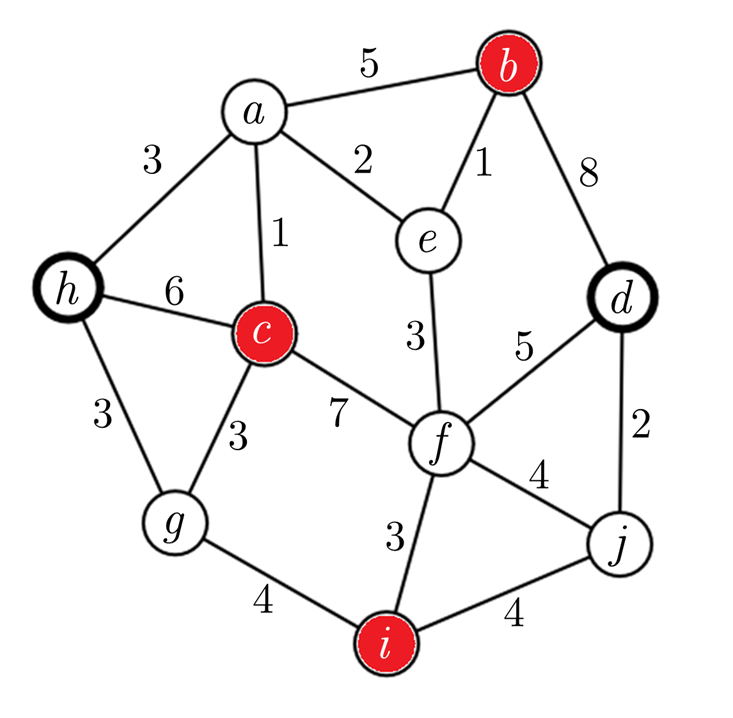
\includegraphics[width=0.35\linewidth]{hotels.png}
\end{figure}

You can spend a maximum of 7 hours each day driving. After traveling \textbf{at most} 7 hours, you must reach a hotel to sleep. From that vertex, you can start driving for another 7 hours the next day. Given a graph $G(V,E)$ and the subset $H$, give a \textbf{polynomial-time} (in $m$ and $n$) algorithm that finds out if it is possible to reach $d$ (starting from $h$) under the 7-hours-per-day constraint. There is no limit on how many days you take. E.g. in the graph shown above, it is possible to travel from $h$ to $d$ under the given constraints using many possible paths, such as $h-g-\textcolor{red}{i}-j-d$ (2 days), or $h-a-e-\textcolor{red}{b}-e-f-\textcolor{red}{i}-j-d$ (3 days). Your algorithm only needs to return yes or no (possibility of reaching $d$), and outputting the number of days and the exact path is not necessary.

It is okay if you do not include a formal proof of correctness. Please give: i) a brief description of your problem-solving approach, ii) the pseudocode, and iii) analysis of the running time. 

\textbf{(i): When I was coming up with an algorithm I realized that we would start by check if $d$ was reachable from $h$ in $\le 7 \text{ steps}$. If it wasn't our only other option would be to visit a hotel. From this hotel we would check if d was reachable in $\le 7 \text{ steps}$. If it was not I would have to use another hotel.}

\textbf{Using this understanding we can create a reachability graph $G' = (N, M)$ such that $N = \{H,h,d\} $ and $(u,v) \in M$ if there exists a path from $u \text{ to } v \le 7 \text{ hours}$ . Once this reachability graph is created we can run BFS to find the minimum number of stops in our reachability graph or DFS if we just want to check if a path exists}

\textbf{(ii): Note - This algorithm assumes that there is a subroutine $\text{Djikstras}(start, end)$ that returns true if there is a path from start to end that has a path cost of $\le 7$. This subroutine is implemented exactly as Djikstras was in class}

\textbf{Note - This algorithm assumes there is a subroutine $\text{BFS}(\text{nodes, edges, start, end})$ that returns true if there exists a path in the graph $G=(nodes, edges)$ between start and end and returns false otherwise. This algorithm is implemented exactly how we saw BFS implemented in class}

\begin{algorithm}
\caption{TripPlanning$(h,d,G,H)$}\label{alg:cap}
\begin{algorithmic}[1]
\State $N \gets H \cup \{h,d\}$ \Comment{Nodes of reachability graph}
\State $M \gets \{\}$ \Comment{Edges of reachability graph} 
\For{every node $u$ in $N$}
\State $\text{dists}[] \gets$ Call Djikstras(u) \Comment{Gives shortest path from u to all v}
\For{every element $a$ in $\text{dists}$}
\State If $a > 7$ discard otherwise add edge $(u, v)$ to reachability graph
\EndFor
\EndFor \\
\Return{$\text{BFS}(N\_r, M\_r, h, d)$}
\end{algorithmic}
\end{algorithm}

\textbf{(iii): }

\textbf{Lines 1-2 are constant}

\textbf{The for loop on lines 3 takes $O(N * logn(m+n))$  where N is the number of hotels + source + destination. The $N$ comes from the fact that we have to run Djikstras for all the values in $N$. The other terms besides the $N$ simply come from the algorithm of Djikstras discussed in class.}

\textbf{The for loop on line 5 takes $O(|N|)$ in the worst case.}

\textbf{Line 10 takes $O(N + M)$ using the usual BFS algorihtm implemented in class}

\textbf{Summing up all of our runtimes we get total runtime which is polynomial}
\begin{align*}
O(N * logn(m+n) * |N| + (N + M)) \\
O(N * logn(m+n))
\end{align*}

\mysolution{
\input{Sol-5}
}

\titledquestion{All-Pairs Shortest Paths (APSP)}
Given a directed graph $G = (V, E)$ with non-negative edge lengths $\{w_e\}$, we define the {\em distance matrix} $M$ as the $n \times n$ matrix ($n = |V|$ as usual) whose $i,j$'th entry is the shortest path distance between vertices $i$ and $j$. Given the graph (vertices, edges and lengths), the goal of the APSP problem is to find the matrix $M$.

In what follows, let $G$ be an {\bf unweighted, undirected} graph (all edge lengths are $1$). Thus, in this case, shortest path from one vertex $u$ to the rest of the vertices can be found via a simple BFS. (Thus the APSP problem can be solved in time $O(n(m+n)) = O(n^3)$.)

Let $A$ denote the {\em adjacency matrix} of the graph, i.e., an $n \times n$ matrix whose $ij$'th entry is $1$ if $ij$ is an edge, and is $0$ otherwise.  Now, consider powers of this matrix $A^k$ (defined by traditional matrix multiplication).  Also, for convenience, define $A^0 = I$ (identity matrix of size $n\times n$). 

\begin{parts}
\part[10] Prove that for any two vertices $i,j$, their distance in the graph $d(i,j)$ is the smallest $k\ge 0$ such that $A^k (i,j) > 0$.\\


\textbf{Claim: For any two vertices $i,j$ their distance in the graph $d(i,j)$ is the smallest $k \ge 0$ such that $A^k(i,j) > 0$. This claim is stating that the first value of $k$ for which the $A^k(i,j) > 0$ represents the shortest distance $d$ between the two vertices $i,j$}

\textbf{We need to prove two facts.}

\textbf{Fact 1: At $k=d: A^k[i,j] > 0$.}

\textbf{Fact 2: At any $k<d: A^k[i,j] = 0$.}

\textbf{We can use induction to prove fact 1.}

\textbf{Base Case: $k=1$. $A^1$ is the adjacency matrix and all non zero entries represent a direct neighbor. There cannot be a shorter path from $[i,j]$ then 1 so the base case is true}

\textbf{Inductive hypothesis. Assume we are given that for all $p < P$ $A^{p-1}[i,j] > 0$ represents the shortest path from $[i,j]$ which is of distance $p-1$}

\textbf{Inductive case. Using our inductive hypothesis and the definition of matrix multiplication we can show that for $p = P$ $A^{P}[i,j] > 0$ represents the shortest path from $[i,j]$ of length $P$. Start with the following.}
\[
A^{P}_{i,j} = \sum_{n}^{k=1} A^{P-1}_{i,k} * A_{k,j}
\]
\textbf{This illustration also demonstrates this fact.}

\begin{figure}[H]
    \centering
    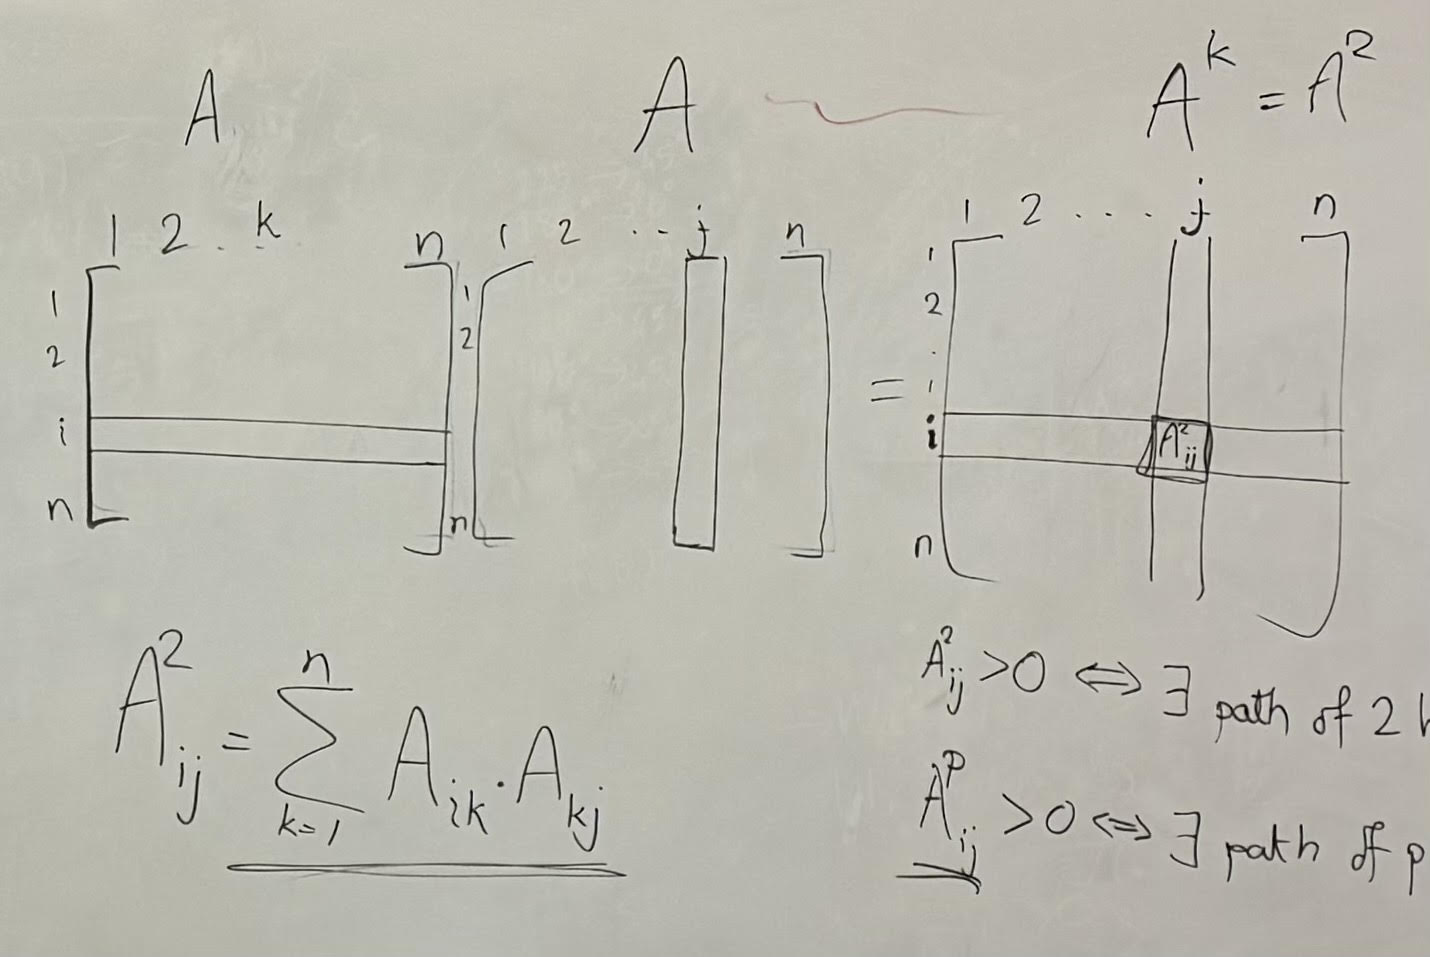
\includegraphics[width=0.5\linewidth]{Matrix Multiplication.jpg}
\end{figure}

\textbf{By our inductivie hypothesis we know that if $A^{P-1}_{i,k} > 0$ then $d(i,k) = P - 1$. We also notcie from the base case that when the other term $A_{k,j} > 0$ that $d(k,j) = 1$. We are trying to show that the left-hand side is $>0$. The left-hand side can only $ > 0$ when both terms on the right hand side are greater than $0$. From this we can find the distance of the path $i$ to $j$ to be $P-1 + 1$ which is exactly $P$. Therefore we have shown that $A^P[i,j] > 0$ represents the shortest path from $[i,j]$ with a distance of $P$. This fact proves our inductive case. We can then put together our base case and our inductive case proofs to prove fact 1 by induction.}

\textbf{We can use contradiction to prove fact 2. Lets assume there is some $k' < d$ such that $A^{k'}[i,j] > 0$. This means that their exists a path of length $k'$ from $[i,j]$. This is a contradiciton because we have already established earlier that the length of the shortest path is $d$ and this claim says that $k' < d$. Therefore fact 2 must be true by contradiction}

\textbf{Having proved fact 1 and fact 2 we have proven that for any two vertices $i,j$, their distance in the graph $d(i,j)$ is the smallest $k \ge 0$ such that $A^k(i,j) > 0$}

\mysolution{
\input{Sol-6a}
}

\part[8] The idea is to now use fast algorithms for computing matrix multiplications. Suppose there is an algorithm that can multiply two $n \times n$ matrices in time $O(n^{2.5})$.  Use this to prove that for any parameter $k$, in $O(k n^{2.5})$ time, we can find $d(i,j)$ for all pairs of vertices $(i,j)$ such that $d(i,j) \le k$.

\mysolution{
\input{Sol-6b}
}

In other words, we can find all the {\em small} entries of the distance matrix. Let us see a different procedure that can handle the ``big'' entries.

\textbf{Provided is pseudocode for the proposed algorithm}

\begin{algorithm}
\caption{Find Shortest Paths}\label{alg:cap}
\begin{algorithmic}[1]
    \State B = I \Comment Let I be the identity matrix
    \For {1 to k}
        \State $B = B * A$
        \State Loop through A and check which entries are non-zero. \Comment These entries are shortest $d(i,j)$
    \EndFor
\end{algorithmic}
\end{algorithm}

\textbf{Line 1 takes constant time}

\textbf{Line 2 is run $k-1$ times we will just say $k$ for simplicity as it doens't change our big-o.}

\textbf{Line 3 takes $O(n^2.5)$ which was given}

\textbf{Line 4 takes $O(n^2)$ loop through each element of the matrix}

\textbf{From this we get a final runtime}
\begin{align*}
    O(k (n^{2.5} + n^2)) \\ 
    O(kn^{2.5} + kn^2) \\
    O(kn^{2.5})
\end{align*}

\textbf{This is a polynomial runtime}

\textbf{Before talking to Yash I also explained the runtime through text. I think that it is much better explained through the psuedo code but I have left it there as "extra work"}

\textbf{Using our proof from (a) we know that for any two vertices $i,j$, their distance in the graph $d(i,j)$ is the smallest  $ k\ge 0$ such that $A^k(i,j) > 0$}
\textbf{The bound $O(kn^2.5)$ simply comes from the matrix multiplication of $A$ to itself. We need to do this $k$ times to find the $A^k$ we are looking for. This $A^k$ gives us $d(i,j)$ for all pairs $\le$ all pairs of $k$. At every step of the matrix multiplication we need to scan our array and keep track of the first time that the entry becomes nonzero. This is because there are cases where we could reach a vertice in $a$ hops but not $a+1$ hops.}


\part[5] Let $i,j$ be two vertices such that $d(i,j) \ge k$.  Prove that if we sample $(2 \ln n) \cdot \frac{n}{k}$ vertices of the graph uniformly at random, the probability of not sampling any vertex on the shortest path from $i$ to $j$ is $\le \frac{1}{n^2}$. [{\em Hint:} You may find the inequality $1-x \le e^{-x}$ helpful.]

\textbf{We start off by defining the probability of failure for a single trial. We know that the shortest path has $k$ hops}
\[
1-\frac{k}{n}
\]
\textbf{If we do this $s$ times the probability of failure for $s$ trials is}
\[
(1-\frac{k}{n})^s
\]
\textbf{Next we can use the hint}
\[
(1-\frac{k}{n})^s \le e^{\frac{k}{n}s}
\]
\textbf{We can simplify the right side}
\setcounter{equation}{0}
\begin{align}
e^{\frac{k}{n}s} = e^{-\frac{k}{n} * 2\ln(n) * \frac{n}{k}} \\
e^{-\frac{k}{n} * 2\ln(n) * \frac{n}{k}} = e^{-2\ln(n)} \\ 
e^{-2ln(n)} = n^{-2}
\end{align}
\textbf{Therefore if we sample $2\ln(n) * \frac{n}{k}$ vertices of the graph uniformly at random, the probability of not smapling any vertex on the shortest path from $i$ to $j$ is $\le \frac{1}{n^2}$}

\mysolution{
\input{Sol-6c}
}
\end{parts}
\end{questions}
\end{document}
